% Created 2021-01-05 二 18:51
% Intended LaTeX compiler: xelatex
\documentclass[11pt]{report}
\usepackage{graphicx}
\usepackage{grffile}
\usepackage{longtable}
\usepackage{wrapfig}
\usepackage{rotating}
\usepackage[normalem]{ulem}
\usepackage{amsmath}
\usepackage{textcomp}
\usepackage{amssymb}
\usepackage{capt-of}
\usepackage{hyperref}
\author{曹嘉祺 PB18030874 化学与材料科学学院 有机化学系 \thanks{中国 安徽合肥 中国科学技术大学 Email: \href{mailto:mkq@mail.ustc.edu.cn}{mkq@mail.ustc.edu.cn}}}
\usepackage[scheme=plain]{ctex}
\usepackage{fontspec}
\usepackage[section]{placeins}
\setmainfont{更纱黑体 UI SC}
\hypersetup{colorlinks=true,linkcolor=blue}
\usepackage{longtable}
\usepackage[version=4]{mhchem}
\def \qCao {C_{A}^{0}}
\def \qCa {C_{A}}
\def \qt {t_{\frac{1}{2}}}
\date{\today}
\title{旋光物质化学反应反应动力学研究}
\hypersetup{
 pdfauthor={曹嘉祺 PB18030874 化学与材料科学学院 有机化学系},
 pdftitle={旋光物质化学反应反应动力学研究},
 pdfkeywords={},
 pdfsubject={},
 pdfcreator={Emacs 27.1 (Org mode 9.4)}, 
 pdflang={English}}
\begin{document}

\maketitle
\tableofcontents

\begin{abstract}
本文介绍了一种利用物理方法来研究化学反应动力学的方法。利用旋光度与浓度的线性关系,通过测定化学反应过程中体系旋光度的变化,可以推算出物质浓度变化与时间的关系,进而可以求出反应的速率常数。同时,通过改变反应物浓度、催化剂的量以及反应温度,可以定性得出上述各项对反应速率的影响,同时通过速率常数与温度的关系可以得到反应的活化能。


\noindent\rule{\textwidth}{0.5pt}
\begin{itemize}
\item 关键词:旋光度 \quad   反应速率常数 \quad      动力学 \quad       蔗糖
\end{itemize}
\end{abstract}
\begin{abstract}
This passage introduces a way to apply the physical properties to study the dynamics of a chemical reaction. Taking advantage of the fact that the optical rotation is linear with concentration, by measuring the change of optical rotation of the system during the chemical reaction, we can calculate the change of concentration with time in the process. Then the reaction rate constant can be got. Meanwhile through altering the concentration of reactant, the amount of the catalyst and the temperature, we can study their influences on reaction rate constant qualitatively; the activation energy can also be calculated.


\noindent\rule{\textwidth}{0.5pt}

\begin{itemize}
\item key words: Optical rotation,reaction rate constant,Dynamics,cane sugar
\end{itemize}
\end{abstract}
\part{前言}
\label{sec:org62cc131}
化学反应动力学研究中有两个非常重要的量,速率常数和半衰期。反应速率是化学反应快慢程度的量度,广义地讲是参与反应的物质的量浓度随时间的变化量的绝对值。半衰期是反应中的反应物消耗掉 50\% 所需的时间;速率常数则为反应反应速率方程中的常数,用k表示。

本实验中,我们利用蔗糖的水解来研究化学反应动力学。蔗糖水解反应可以视为一级反应。由于旋光性与反应物质的浓度要有简单的线性关系,并且在反应过程中反应体系的旋光性要有明显的变化,且旋光性易于测量,因而测定反应进程中某一时刻反应物或产物的浓度

在本实验中,我们根据反应物与生成物均含有不对称碳原子,它们都具有旋光性,但旋光能力不同这一特点,可用体系反应过程旋光度的变化来量度反应的进程。

\chapter{实验目的与要求}
\label{sec:orgc45fed1}
\begin{enumerate}
\item 测定蔗糖转化反应的速率常数和半衰期。
\item 了解反应物浓度与旋光度之间的关系。
\item 了解旋光仪的基本原理,掌握旋光仪的正确使用。
\end{enumerate}
\chapter{实验原理}
\label{sec:orgdbeb670}
反应速率只与某反应物浓度成正比的反应称为一级反应,即:
\[
-\frac{d\qCa}{d t}=k\qCa
\]
式中:\(k\) 是反应速率常数,\(\qCa\) 是反应物的浓度,\(t\) 是时间,设\(\qCao\) 为反应物起始浓度,
积分可得:
\[
\ln\qCa = -kt+\ln \qCao
\]
若以\(\ln \qCa\) 对t作图,可得一直线,其斜率的绝对值即为反应速度常数\(k\) .

反应速度还可用半衰期
\(\qt\) 来表示。若为在\(t\) 时间内已经起反应了的反应物浓度,则在\(t\) 时的反应速度为:
\[
-\frac{d(\qCao -x)}{dt}=k(\qCao -x)
\]
积分可得:
\[
t=\frac{1}{k}\ln\frac{\qCao}{\qCao -x}
\]

当反应物浓度为起始浓度一半时,即:
\[
x=\frac{1}{2}\qCao
\]
时所需之时间,称为半衰期\(\qt\) ,显然:
\[
\qt =\frac{1}{k}\ln\frac{\qCao}{\qCao -\frac{1}{2}\qCao} =\frac{\ln 2}{k} =\frac{0.693}{k}
\]
上式说明一级反应的半衰期只决定于反应速度常数\(k\) ,而与起始浓度无关。这是一级反应的一个特点。  
蔗糖转化的反应方程式为:
\[
\underset{蔗糖}{\ce{C12H22O11}} \ce{ + H2O ->T[H+]} \underset{葡萄糖}{\ce{C6H12O6}} + \underset{果糖}{\ce{C6H12O6}}}
\]

此反应的反应速度与蔗糖的浓度、水的浓度以及催化剂\(H^{+}\) 的浓度有关。在催化剂\(H^{+}\) 浓度固定的条件下,
这个反应本是二级反应,但由于有大量水存在,
虽然有部分水分子参加反应,但在反应过程中水的浓度变化极小。因此,反应速度只与蔗糖浓度成正比。其浓度与时间的关系,符合反应速率只与某反应物浓度成正比的条件,
所以此反应为一级反应。若在反应过程中的不同时间测得蔗糖的相应浓度,
代入上式即可求得该反应的速度常数\(k\) 。

测定反应进程中某一时刻反应物或产物的浓度有两种方法:
\begin{enumerate}
\item 化学方法是在反应过程中每经过一定的时间取出部分反应混合物,并用化学的方法使其反应立即停止,记录时间,分析此时反应混合物中产物或反应物的浓度。这种方法得到的结果比较准确,重复性较好,但操作的手续较为繁琐,有些反应让其中止比较困难。
\item 物理方法是利用反应体系中反应物或产物的某些物理性质(例如导电性、旋光性、吸光、体积、压力、折光等)与物质浓度的关系,通过测量这些物理性质的变化来确立物质的浓度。用物理方法进行测量时要满足以下条件:
\begin{itemize}
\item 物理性质与反应物质的浓度要有简单的线性关系,最好是正比关系。
\item 在反应过程中反应体系的物理性质要有明显的变化。
\item 不能有干扰因素。
\item 有较好的测量仪器设备。
\end{itemize}
\end{enumerate}

物理法的优点在于不需从反应体系中取出样品,可直接测定,它不需要停止反应而可连续迅速地进行分析,且可将物理性质变成电信号进行自动记录等。但对于那些反应中有副反应或少量杂质对所测量的物理性质影响较灵敏时将会造成较大的误差。

本实验是根据反应物与生成物均含有不对称碳原子,它们都具有旋光性,但旋光能力不同这一特点,可用体系反应过程旋光度的变化来量度反应的进程。

测量旋光度所用的仪器称为旋光仪。溶液的旋光度与溶液中所含有旋光物质之旋光能力、溶剂的性质、溶液的浓度、样品管长度、光源波长及温度等均有关系。当其它条件固定时,旋光度与反应物浓度\(C\) 呈线性关系,即:
\[
\alpha = KC
\]
式中\(K\) 与物质旋光能力、溶剂性质、样品管长度、温度等有关。

物质的旋光能力用比旋光度来度量。比旋光度可用下式表示:
\[
[\alpha]_{D}^{t}=\frac{\alpha\cdot 100}{IC}
\]
式中:
\begin{itemize}
\item t:实验温度。
\item D:所用光源为钠灯D线(波长589nm)。
\item \(\alpha\):测得的旋光度(\textsuperscript{o})。
\item l:样品管的长度(dm)。
\item C:浓度(g/100mL)。
\end{itemize}

作为反应物的蔗糖是右旋性的物质,
其比旋光度\([\alpha]_{D}^{20}=66.6^{o}\) 。
生成物中,葡萄糖也是右旋性的物质,其比旋度\([\alpha]_{D}^{20}=52.5^{o}\) 。但果糖是左旋性物质,其比旋度\([\alpha]_{D}^{20}=-91.9^{o}\) 。
由于生成物中果糖之左旋比葡萄糖右旋性大,所以生成物呈左旋性质。
因此,随着反应的进行,体系的右旋角不断减小。反应至某一瞬间,体系的旋光度可恰好等于零,而后就变成左旋,直至蔗糖完全转化,这时左旋角达到最大值\(\alpha_{\infty}\) 。设体系最初的旋光度为\(\alpha_{0}\) ,则
\[
\alpha_{0}=K_{反}\qCao (t=0,蔗糖未转化)
\]
最终体系的旋光度为:
\[
\alpha_{\infty}=K_{生}\qCao (t=\infty,蔗糖完全转化)
\]
式中,\(K_{反}\) 和\(K_{生}\) 分别为反应物与生成物之比例常数。当时间为\(t\) 时,
蔗糖浓度为\(\qCa\) ,此时旋光度\(\alpha_{t}\) 为:
\[
\alpha_{t}=K_{反}\qCa+K_{生}(\qCao-\qCa)
\]
综合上面几式可得:
\[
\qCao=\frac{\alpha_{0}-\alpha_{\infty}}{K_{反}-K_{生}}=K'(\alpha_{0}-\alpha_{\infty})
\]
\[
\qCa=\frac{\alpha_{t}-\alpha_{\infty}}{K_{反}-K_{生}}=K'(\alpha_{t}-\alpha_{\infty})
\]
代入积分式后,得:
\[
\ln(\alpha_{t}-\alpha_{\infty})=-kt+\ln(\alpha_{0}-\alpha_{\infty})
\]
若以\(\ln(\alpha_{t}-\alpha_{\infty})\) 对\(t\) 作图,得一直线,其斜率为\(-k\) ,从而求得反应的速度常数\(k\) .

\part{实验部分}
\label{sec:org27f19fc}
\chapter{实验仪器与试剂}
\label{sec:org7ab145e}
\begin{center}
\begin{tabular}{ll}
仪器 & 备注\\
\hline
WZZ-2B自动旋光仪 & 上海精密科学仪器有限公司\\
HK-2A超级恒温水浴 & 南京南大万和科技有限公司\\
电子天平 & \\
锥形瓶 & \\
移液管 & 25ml,50ml\\
广口瓶 & \\
蔗糖 & AR\\
盐酸 & 4mol/L\\
\end{tabular}
\end{center}

\chapter{实验步骤}
\label{sec:org6856cd8}
\begin{enumerate}
\item 了解、熟悉旋光仪的结构、原理和使用方法。
\item 用蒸馏水校正仪器的零点,蒸馏水为非旋光物质,可用以校正仪器的零点(即\(\alpha=0\) 时仪器对应的刻度)。校正时,先冼净样品管,将管一端加上盖子,并向管内灌满蒸馏水,使液体形成一凸出了液面,然后在样品管上面盖上玻璃片,此时管内不应有气泡存在,再旋上套盖,使玻璃片紧贴于旋光管,勿使漏水。但必须注意旋紧套盖时不能用力过猛,以免玻璃片压碎。用滤纸将样品管擦干,再用擦镜纸将样品管两端的玻璃片擦干净。将样品管放入旋光仪内。打开光源,调整目镜聚焦,使视野清楚。然后旋转检偏镜,直到所观察到的三分视野暗度相等为止,记下检偏镜之旋角,重复测量数次,取其平均值,此均值即为零点,用来校正仪器的系统误差。(但实际上是用空气和石英校正的)
\item 蔗糖转化旋光度的测定:将超级恒温槽调节到所需的温度,在干燥的150mL的锥形瓶中准确移取25ml蔗糖溶液,在另一试剂瓶中置入一些4 mol\(\cdot\) dm\textsuperscript{-3} HCl,将两只锥形瓶都放入超级恒温水浴的恒温箱内,恒温至少半小时,然后准确移取25mL已恒温的HCl,注入到已恒温的25mL蔗糖溶液中,待移液管中的HCl流出一半时开始记时,将混合的的反应物摇匀,迅速用少量反应液洗涤样品管2-3次,然后将反应液装满样品管,盖好盖子并擦净。立即放入旋光仪内,测量各时间的旋光度。第一个数据要求离开始起反应的3min内记录,测量时将三分视野调节暗度相等后,先记录时间,再读取旋光度。为了多读一些数据,反应开始15min内,每分钟测量一次,以后由于反应物浓度降低,一直测量到出现旋光度负值为止。反应速度变慢,可以将每次测量的时间间隔适当放长。
\end{enumerate}

\chapter{实验数据及数据处理(见附件)}
\label{sec:org6e55f4e}
\chapter{结果分析与讨论}
\label{sec:org523e851}
\section{实验结果}
\label{sec:orgc94c449}
\begin{enumerate}
\item 本人实验结果
\label{sec:org7ec2fc7}
\begin{enumerate}
\item 旋光度-时间图像
\label{sec:org35210d2}
\begin{enumerate}
\item 35\textsuperscript{o}C
\label{sec:org9d1fe47}
\begin{center}
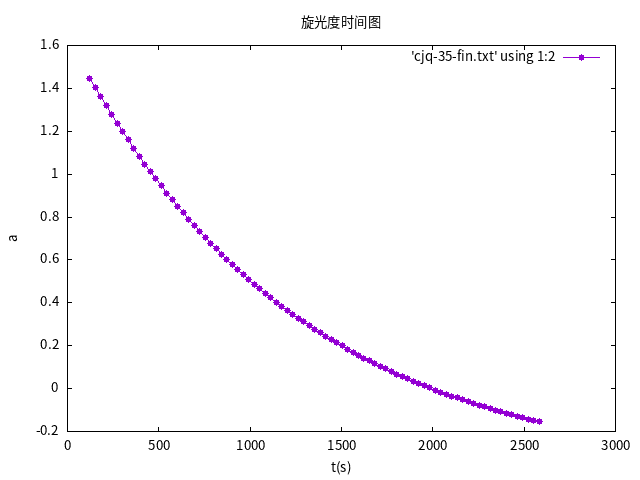
\includegraphics[width=.9\linewidth]{../data/cjq-35.png}
\end{center}
\item 40\textsuperscript{o}C
\label{sec:orgdf4b667}
\begin{center}
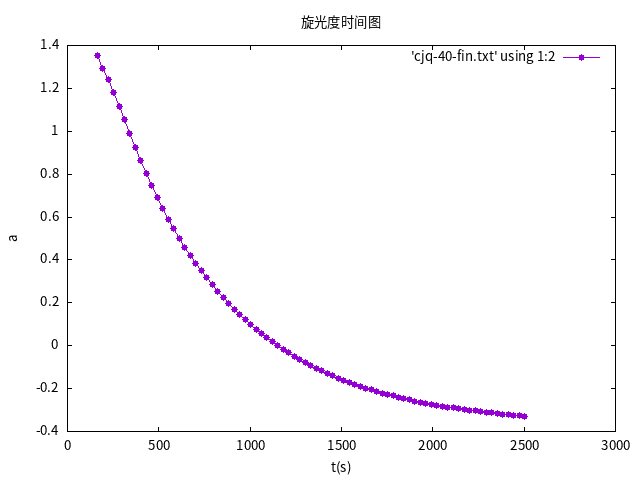
\includegraphics[width=.9\linewidth]{../data/cjq-40.png}
\end{center}
\end{enumerate}
\item 旋光度对数-时间图像
\label{sec:orgb40f77c}
\begin{enumerate}
\item 35\textsuperscript{o}C
\label{sec:org0907b29}
\begin{center}
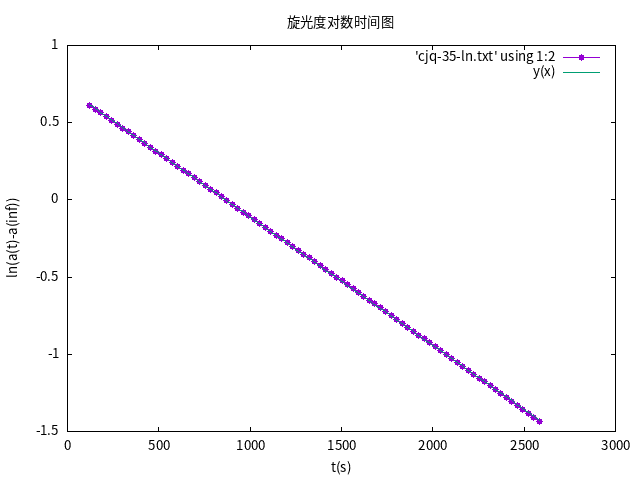
\includegraphics[width=.9\linewidth]{../data/cjq-35-ln.png}
\end{center}
拟合直线的斜率k为-0.000830,所以
\[
t_{1/2}=\frac{\ln 2}{|k|}=\frac{\ln 2}{0.000830}=835.12(s)
\]
\item 40\textsuperscript{o}C
\label{sec:orgb0cfb86}
\begin{center}
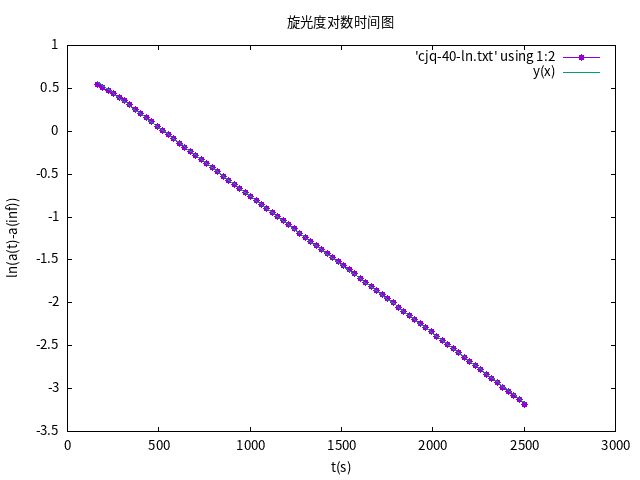
\includegraphics[width=.9\linewidth]{../data/cjq-40-ln.png}
\end{center}
拟合直线的斜率k为-0.001600(s\textsuperscript{-1}),所以
\[
t_{1/2}=\frac{\ln 2}{|k|}=\frac{\ln 2}{0.001600}=433.22(s)
\]
\end{enumerate}

\item 表观活化能的计算
\label{sec:org7594772}
\[
E_{a}=-\frac{R\ln \frac{k_{1}}{k_{2}}}{\frac{1}{T_{2}}-\frac{1}{T_{1}}}=-\frac{R\cdot \ln\frac{0.001600}{0.000830}}{\frac{1}{273.15+40}-\frac{1}{273.15+35}}=105.312(kJ\cdot mol^{-1})
\]
\end{enumerate}
\item 小组实验结果
\label{sec:org1d1d42f}
小组同学实验结果汇总如下:
\begin{center}
\begin{tabular}{lrrrrrr}
组别 & T(\textsuperscript{o}C) & 蔗糖(10g/L) & HCl(mol/L) & k(s\textsuperscript{-1}) & \(\qt\) (s) & \(E_{a}\) (kJ/mol)\\
\hline
1(向思佳) & 30 & 5 & 2 & 0.000381 & 1812.0 & 97.214\\
2(向思佳) & 40 & 5 & 2 & 0.001304 & 468.0 & 97.214\\
3(艾姆拉) & 30 & 10 & 4 & 0.001730 & 400.8 & 85.399\\
4(艾姆拉) & 35 & 10 & 4 & 0.002998 & 231.0 & 85.399\\
5(刘煜超) & 30 & 5 & 4 & 0.001350 & 513.4 & 110.970\\
6(刘煜超) & 35 & 5 & 4 & 0.002760 & 291.7 & 110.970\\
7(周靖辰) & 30 & 10 & 2 & 0.000509 & 1362.6 & 129.500\\
8(周靖辰) & 35 & 10 & 2 & 0.001172 & 591.5 & 129.500\\
9(曹嘉祺) & 35 & 5 & 2 & 0.000830 & 834.0 & 105.312\\
10(曹嘉祺) & 40 & 5 & 2 & 0.001600 & 433.2 & 105.312\\
\end{tabular}
\end{center}
\[
\overline{E_{a}}=105.679kJ\cdot mol^{-1}
\]

\item 结果讨论
\label{sec:org4eef8ca}

\begin{enumerate}
\item 盐酸浓度影响(1,5|7,3|9,6|8,4)
\label{sec:org5cf5993}
\begin{enumerate}
\item 在同浓度底物同温度下,可以明显发现随着HCl浓度升高,化学反应速率常数升高。且盐酸浓度增大一倍,k值增大3倍左右。
由此可见,在实验条件下,盐酸浓度对速率常数的影响可能还与温度蔗糖浓度等因素有关。但毋庸置疑的一点是反应速率确实随盐酸浓度增大而增大了, 这可能是由于盐酸是反应的催化剂,催化剂的用量不同,也会影响反应的速率常数
\item 理论上增加酸浓度活化能也会降低,但在实验中未观察到。
\end{enumerate}
\item 温度的影响(1,9,2|5,6|7,8|3,4)
\label{sec:org608296a}
\begin{enumerate}
\item 在相同底物和HCl浓度条件下,可明显观察到随着温度的升高,化学反应速率常数也升高。
\item 根据阿伦尼乌斯公式
\[
	 k=A\cdot e^{\frac{-E_{a}}{RT}}
	 \]
由于温度位于指数的分母上,温度越大,指数项越大,速率常数越大。
\item 根据对数据的观察,温度每升高\(5^{o}C\) 反应速率提高一倍左右
\end{enumerate}
\item 蔗糖浓度的影响(1,7|5,3|9,8|6,4)
\label{sec:org84ada07}
\begin{enumerate}
\item 在相同温度相同浓度HCl条件下,可发现随着底物浓度的改变,化学反应速率常数基本不变。
\item 但反应速率发生改变,浓度越大,速率越快,这可由旋光度随时间变化的快慢看出,理论原因是由于蔗糖转化反应是一级反应,反应速率与反应物的浓度成正比
\end{enumerate}
\item 讨论
\label{sec:orgf188429}
\begin{enumerate}
\item 由数据处理过程可知,\(\ln(\alpha_{t}-\alpha_{\infty})\sim t\) 曲线的线性拟合度都很高,这也证明了在实验条件下,HCl浓度一定时,该反应是一级反应。
\item 实验中活化能的测定是结合五个人的数据计算的,由于操作人员、实验仪器等的差异,会有较大的误差。实验结果基本在105.7kJ/mol左右,与理论值107kJ/mol较接近。而且实际上活化能与酸度相关,故而酸度的差异也会造成与理论值的差异。
\item 如上所述,实验中没有明显观察到活化能随酸度升高而降低,这也是不同实验人员不同仪器造成的差异。
\end{enumerate}
\end{enumerate}
\end{enumerate}

\section{实验讨论}
\label{sec:org8537467}
\begin{enumerate}
\item 误差分析
\label{sec:org9f7058b}
\begin{enumerate}
\item 如上所述,引起最大误差的原因是不同人员的实验习惯以及不同仪器自身的差异所造成的。
\item 实验中不同同学是采取不同的方式(如混合后摇晃的次数就有所不同)混合底物和酸的,这会造成反应速率的测定时的一些误差
\item 在混合样品的过程中,溶液温度会降低,故而开始时的数据会受到影响。
\item 实验过程中发现,尤其对于高酸组,由于反应很快,示数迅速降低,很难稳定,这会对读数造成较大误差。
\item 对于高糖高酸组,在测定充分反应旋光度时,由于加热时间过长,蔗糖发生了碳化,溶液的颜色改变无疑会影响旋光度的测量
\item 实际上\(\alpha_{\infty}\) 在每一组处理数据中都会用到,会对实验结果有较大影响,而如上分析,可能在测量时溶液中蔗糖尚未反应完全。
\end{enumerate}
\item 实验思考
\label{sec:orgb49090e}
\begin{enumerate}
\item 查阅文献可知,蔗糖水解反应并非那样简单,而是复杂得多。
对转化过程而言,最多称它为准(或假)一级反应。除非溶液很稀,
利用一级反应速度方程而得到的\(k\) 值并非常数,
随着水解的进程呈稳步增加。但也非
\[
	r=k[糖][水]
	\]
的二级反应。水解的速度可被表达为
\[
	-\frac{dc}{dt}=k'\frac{[糖]}{[水]}a_{H^{+}}
	\]
水量的减少和氢离子活度的增大,就成为一级反应速度常数稳步增加的原因。
作为基础反应,我们仍将其视为一级反应处理,这并不引入多大的误差,
当蔗糖浓度不大时结果仍将令人满意。
\item 查阅文献可知:蔗糖的水解在酸性介质中进行,\(H^{+}\) 为催化剂,在\([H^{+}]\) 浓度较低时,
水解速度\(k\propto [H^{+}]\) 但在\([H^{+}]\) 增加时,\(k\) 与\([H^{+}]\) 不成比例,且用\(HCl\) 和用\(HNO_{3}\) 或\(HClO_{4}\) 对反应速度常数的影响也不一样(特别是酸浓度高时)。进一步实验指出若\([H^{+}]\) 较大,反应速度常数\(k\) 正比于\(h_{0}\) ,而\(h_{0}\) 可予如下定义:
\[
	h_{0}=a_{H^{+}}+\frac{\gamma_{S}}{\gamma_{SH^{+}}}
	\]
其中\(a_{H^{+}}\) 是氢离子活度,\(\gamma_{S}\) 和\(\gamma_{SH^{+}}\) 为\(H^{+}\) 、\(SH^{+}\) 的活度系数,其中\(S\) 代表蔗糖,利用\([H^{+}]\) 对\(k\) 的影响,可以研究蔗糖水解的机理,长期以来有二种假设:
\[
	\ce{S + H^+ <=>T[快] SH^+}\quad \ce{SH^+ ->T[慢] x^+ } \quad \ce{x^+ + H2O ->T[快] P + H^+ }
	\]
另一个为
\[
	\ce{S + H^+ <=>T[快] SH^+}\quad \ce{SH^+ + H2O ->T[慢]  P + H^+ }
	\]
按照第一种机理属一级反应,从理论上可以推出反应速度常数\(k\) 应与\(h_{0}\) 成正比,按照第二种机理反应属假单分子(二级)反应,从理论上可以推出反应速度常数\(k\) 应与\([H^{+}]\) 成正比。从而实践证明第一种机理是正确的,因而蔗糖水解判为一级反应。
反应是一复杂反应。显然其计量方程式并不表示此反应的机理,反应也非双分子反应。
\item 本实验中所用的无机酸催化剂对旋光仪有强腐蚀性,会缩短仪器的正常使用时间;测试废液如果不进行处理就直接排放会对环境造成污染。针对实验中存在的这些不足, 可用强酸性阳离子树脂代替无机酸催化蔗糖水解,通过测定旋光度求得催化反应速率常数和活化能。实验结果表明:强酸性阳离子树脂催化蔗糖水解反应能达到与无机酸催化相同的实验效果,
而且实验使用过的树脂经水洗涤后可循环使用。
\end{enumerate}
\end{enumerate}
\part{参考文献}
\label{sec:org259d42b}
\begin{enumerate}
\item 【物理化学】(下册)傅献彩等,高等教育出版社
\item 【物理化学】(美)V.弗里德等著 高等教育出版社, 1983年7月
\item 【展望21世纪的化学】王佛松等主编,化学工业出版社,2000年5月
\item Walter J.moore. “Physical Chemistry”.4tth ed. 253\textasciitilde{}254(1963)
\item Worley. J. Chem .SOC. 99, 349(1911)
\item Pennycuick. J. Am. Chm. Soc. 48, 6(1926)
\end{enumerate}

\part{附录: 数据处理过程}
\label{sec:orgc8871bc}
以下数据处理过程仅涉及本人的数据,其他同学的数据请参阅他们的实验报告
\chapter{原始数据}
\label{sec:org60aa4be}
以下的数据均以计入从混合到仪器启动这个过程所用的时间,在35\textsuperscript{o}C下这个时间为123s,在40\textsuperscript{o}C下为162s.
\section{35\textsuperscript{o}C下的时间-旋光度数据}
\label{sec:org1ac3f67}
\begin{center}
\begin{tabular}{rrrrrrrr}
时间(s) & 旋光度 & 时间(s) & 旋光度 & 时间(s) & 旋光度 & 时间(s) & 旋光度\\
\hline
123 & 1.4461 & 723 & 0.7321 & 1323 & 0.2935 & 1923 & 0.0235\\
153 & 1.4048 & 753 & 0.7048 & 1353 & 0.2766 & 1953 & 0.0135\\
183 & 1.3627 & 783 & 0.6789 & 1383 & 0.2608 & 1983 & 0.0031\\
213 & 1.3190 & 813 & 0.6528 & 1413 & 0.2446 & 2013 & -0.0066\\
243 & 1.2777 & 843 & 0.6266 & 1443 & 0.2290 & 2043 & -0.0164\\
273 & 1.2371 & 873 & 0.6025 & 1473 & 0.2138 & 2073 & -0.0257\\
303 & 1.1987 & 903 & 0.5783 & 1503 & 0.1988 & 2103 & -0.0350\\
333 & 1.1596 & 933 & 0.5547 & 1533 & 0.1843 & 2133 & -0.0437\\
363 & 1.1203 & 963 & 0.5307 & 1563 & 0.1699 & 2163 & -0.0526\\
393 & 1.0833 & 993 & 0.5083 & 1593 & 0.1561 & 2193 & -0.0611\\
423 & 1.0472 & 1023 & 0.4870 & 1623 & 0.1426 & 2223 & -0.0694\\
453 & 1.0132 & 1053 & 0.4648 & 1653 & 0.1293 & 2253 & -0.0775\\
483 & 0.9776 & 1083 & 0.4439 & 1683 & 0.1166 & 2283 & -0.0854\\
513 & 0.9454 & 1113 & 0.4235 & 1713 & 0.1039 & 2313 & -0.0931\\
543 & 0.9116 & 1143 & 0.4034 & 1743 & 0.0916 & 2343 & -0.1008\\
573 & 0.8808 & 1173 & 0.3840 & 1773 & 0.0793 & 2373 & -0.1082\\
603 & 0.8487 & 1203 & 0.3650 & 1803 & 0.0679 & 2403 & -0.1149\\
633 & 0.8195 & 1233 & 0.3465 & 1833 & 0.0565 & 2433 & -0.1223\\
663 & 0.7901 & 1263 & 0.3290 & 1863 & 0.0454 & 2463 & -0.1292\\
693 & 0.7613 & 1293 & 0.3113 & 1893 & 0.0344 & 2493 & -0.1358\\
 &  &  &  &  &  & 2523 & -0.1424\\
 &  &  &  &  &  & 2553 & -0.1486\\
 &  &  &  &  &  & 2583 & -0.1549\\
\end{tabular}
\end{center}
\section{40\textsuperscript{o}C下的时间-旋光度数据}
\label{sec:org7fb9288}
\begin{center}
\begin{tabular}{rrrrrrrr}
时间(s) & 旋光度 & 时间(s) & 旋光度 & 时间(s) & 旋光度 & 时间(s) & 旋光度\\
\hline
162 & 1.3553 & 732 & 0.3505 & 1332 & -0.0917 & 1932 & -0.2628\\
192 & 1.2911 & 762 & 0.3160 & 1362 & -0.1045 & 1962 & -0.2681\\
222 & 1.2395 & 792 & 0.2853 & 1392 & -0.1170 & 1992 & -0.2729\\
252 & 1.1800 & 822 & 0.2538 & 1422 & -0.1286 & 2022 & -0.2775\\
282 & 1.1175 & 852 & 0.2240 & 1452 & -0.1399 & 2052 & -0.2819\\
312 & 1.0544 & 882 & 0.1973 & 1482 & -0.1506 & 2082 & -0.2861\\
342 & 0.9903 & 912 & 0.1702 & 1512 & -0.1608 & 2112 & -0.2900\\
372 & 0.9258 & 942 & 0.1460 & 1542 & -0.1705 & 2142 & -0.2936\\
402 & 0.8630 & 972 & 0.1222 & 1572 & -0.1798 & 2172 & -0.2974\\
432 & 0.8029 & 1002 & 0.0993 & 1602 & -0.1890 & 2202 & -0.3008\\
462 & 0.7458 & 1032 & 0.0776 & 1632 & -0.1973 & 2232 & -0.3040\\
492 & 0.6910 & 1062 & 0.0569 & 1662 & -0.2054 & 2262 & -0.3072\\
522 & 0.6395 & 1092 & 0.0371 & 1692 & -0.2131 & 2292 & -0.3104\\
552 & 0.5908 & 1122 & 0.0183 & 1722 & -0.2206 & 2322 & -0.3132\\
582 & 0.5449 & 1152 & 0.0002 & 1752 & -0.2270 & 2352 & -0.3158\\
612 & 0.5015 & 1182 & -0.0169 & 1782 & -0.2342 & 2382 & -0.3186\\
642 & 0.4603 & 1212 & -0.0333 & 1812 & -0.2405 & 2412 & -0.3209\\
672 & 0.4215 & 1242 & -0.0491 & 1842 & -0.2467 & 2442 & -0.3233\\
702 & 0.3834 & 1272 & -0.0640 & 1872 & -0.2523 & 2472 & -0.3255\\
 &  & 1302 & -0.0781 & 1902 & -0.2578 & 2502 & -0.3278\\
\end{tabular}
\end{center}

\section{35\textsuperscript{o}C充分反应}
\label{sec:org5706933}
\begin{center}
\begin{tabular}{rr}
时间 & 旋光度\\
\hline
5:48:09 & -0.4096\\
5:48:37 & -0.3961\\
5:49:07 & -0.3918\\
5:49:37 & -0.3893\\
5:50:07 & -0.3899\\
5:50:37 & -0.3903\\
5:51:07 & -0.3906\\
5:51:37 & -0.3909\\
5:52:06 & -0.3911\\
5:52:36 & -0.3911\\
5:53:07 & -0.3914\\
5:53:37 & -0.3915\\
5:54:07 & -0.3917\\
5:54:37 & -0.3921\\
5:55:07 & -0.3923\\
5:55:37 & -0.3927\\
5:56:06 & -0.3930\\
\end{tabular}
\end{center}
\section{40\textsuperscript{o}C充分反应}
\label{sec:org562596b}
\begin{center}
\begin{tabular}{rr}
时间 & 旋光度\\
\hline
6:01:45 & -0.4085\\
6:02:15 & -0.4050\\
6:02:45 & -0.3931\\
6:03:15 & -0.3834\\
6:03:45 & -0.3753\\
6:04:15 & -0.3714\\
6:04:45 & -0.3682\\
6:05:16 & -0.3673\\
6:05:46 & -0.3707\\
6:06:16 & -0.3691\\
6:06:46 & -0.3695\\
6:07:16 & -0.3694\\
6:07:46 & -0.3693\\
6:08:16 & -0.3693\\
6:08:46 & -0.3693\\
6:09:14 & -0.3692\\
6:09:46 & -0.3692\\
6:10:14 & -0.3693\\
\end{tabular}
\end{center}
\chapter{数据处理}
\label{sec:org0ddd398}
取\(35^{o}C\) 时的\(\alpha_{\infty}\) 为-0.3930,
取\(40^{o}C\) 时的\(\alpha_{\infty}\) 为-0.3693.
\section{旋光度-时间图像}
\label{sec:orge0804ec}
直接利用原始数据将旋光度对时间作图
\begin{enumerate}
\item 35\textsuperscript{o}C
\label{sec:org0280c4d}
\begin{center}
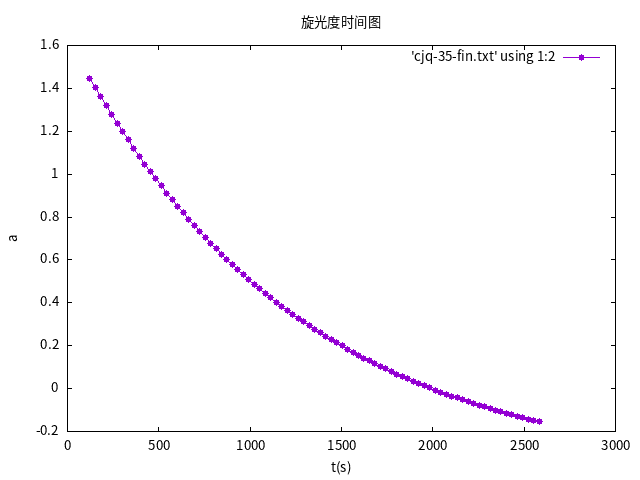
\includegraphics[width=.9\linewidth]{../data/cjq-35.png}
\end{center}
\item 40\textsuperscript{o}C
\label{sec:orgf32cae2}
\begin{center}
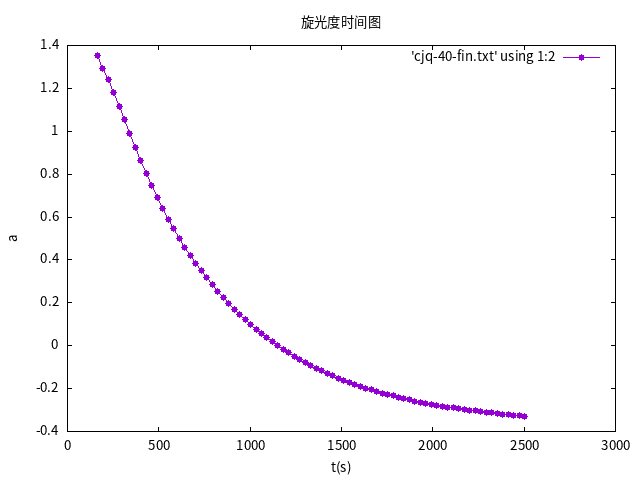
\includegraphics[width=.9\linewidth]{../data/cjq-40.png}
\end{center}
\end{enumerate}
\section{旋光度对数-时间图像}
\label{sec:org1611138}
将上表中旋光度一项进行处理改为\(ln(\alpha_{t}-\alpha_{\infty})\) ,得到的表格数据并作图如下
\begin{enumerate}
\item 35\textsuperscript{o}C
\label{sec:org87468fc}
\begin{center}
\begin{tabular}{rrrrrrrr}
时间 & ln(a\textsubscript{t}-a\textsubscript{\(\infty\)}) & 时间 & ln(a\textsubscript{t}-a\textsubscript{\(\infty\)}) & 时间 & ln(a\textsubscript{t}-a\textsubscript{\(\infty\)}) & 时间 & ln(a\textsubscript{t}-a\textsubscript{\(\infty\)})\\
\hline
123 & 0.609276 & 723 & 0.117872 & 1323 & -0.376149 & 1923 & -0.875869\\
153 & 0.586564 & 753 & 0.093308 & 1353 & -0.401075 & 1953 & -0.900171\\
183 & 0.562868 & 783 & 0.069433 & 1383 & -0.424954 & 1983 & -0.926089\\
213 & 0.537662 & 813 & 0.044782 & 1413 & -0.450044 & 2013 & -0.950882\\
243 & 0.513243 & 843 & 0.019410 & 1443 & -0.474815 & 2043 & -0.976572\\
273 & 0.488641 & 873 & -0.004510 & 1473 & -0.499556 & 2073 & -1.00158\\
303 & 0.464803 & 903 & -0.029120 & 1503 & -0.524587 & 2103 & -1.02722\\
333 & 0.439931 & 933 & -0.053717 & 1533 & -0.549393 & 2133 & -1.05182\\
363 & 0.414293 & 963 & -0.079368 & 1563 & -0.574653 & 2163 & -1.07763\\
393 & 0.389539 & 993 & -0.103917 & 1593 & -0.599475 & 2193 & -1.10292\\
423 & 0.364782 & 1023 & -0.127833 & 1623 & -0.624368 & 2223 & -1.12825\\
453 & 0.340891 & 1053 & -0.153384 & 1653 & -0.649513 & 2253 & -1.15360\\
483 & 0.315249 & 1083 & -0.178051 & 1683 & -0.674129 & 2283 & -1.17896\\
513 & 0.291475 & 1113 & -0.202728 & 1713 & -0.699366 & 2313 & -1.20431\\
543 & 0.265896 & 1143 & -0.227654 & 1743 & -0.724431 & 2343 & -1.23032\\
573 & 0.242005 & 1173 & -0.252315 & 1773 & -0.750141 & 2373 & -1.25597\\
603 & 0.216481 & 1203 & -0.277072 & 1803 & -0.774574 & 2403 & -1.27977\\
633 & 0.192684 & 1233 & -0.301781 & 1833 & -0.799619 & 2433 & -1.30674\\
663 & 0.168138 & 1263 & -0.325730 & 1863 & -0.824624 & 2463 & -1.33256\\
693 & 0.143494 & 1293 & -0.350551 & 1893 & -0.850035 & 2493 & -1.35790\\
 &  &  &  &  &  & 2523 & -1.38390\\
 &  &  &  &  &  & 2553 & -1.40895\\
 &  &  &  &  &  & 2583 & -1.43506\\
\end{tabular}
\end{center}
作图如下:
\begin{center}
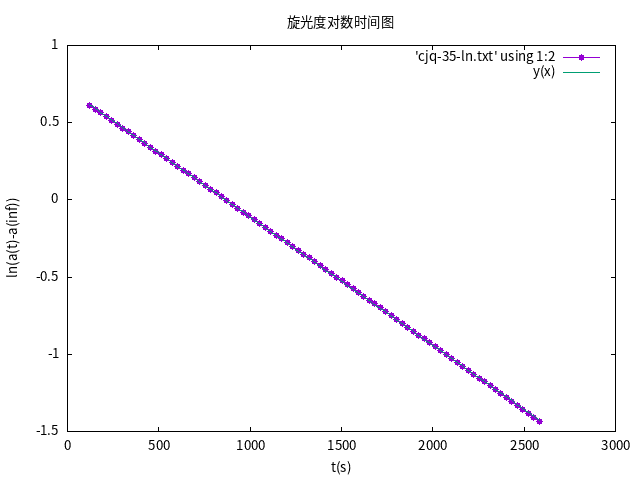
\includegraphics[width=.9\linewidth]{../data/cjq-35-ln.png}
\end{center}
拟合结果如下:
\begin{verbatim}
After 6 iterations the fit converged.
final sum of squares of residuals : 0.00104755
rel. change during last iteration : -1.53832e-06

degrees of freedom    (FIT_NDF)                        : 81
rms of residuals      (FIT_STDFIT) = sqrt(WSSR/ndf)    : 0.00359621
variance of residuals (reduced chisquare) = WSSR/ndf   : 1.29327e-05

Final set of parameters            Asymptotic Standard Error
=======================            ==========================
k               = -0.000830274     +/- 5.492e-07    (0.06615%)
b               = 0.718933         +/- 0.0008414    (0.117%)

correlation matrix of the fit parameters:
#                k      b      
k               1.000 
b              -0.883  1.000 

\end{verbatim}
拟合直线的斜率k为-0.000830,所以
\[
t_{1/2}=\frac{\ln 2}{|k|}=\frac{\ln 2}{0.000830}=835.12(s)
\]
\item 40\textsuperscript{o}C
\label{sec:org0705058}
\begin{center}
\begin{tabular}{rrrrrrrr}
时间 & ln(a\textsubscript{t}-a\textsubscript{\(\infty\)}) & 时间 & ln(a\textsubscript{t}-a\textsubscript{\(\infty\)}) & 时间 & ln(a\textsubscript{t}-a\textsubscript{\(\infty\)}) & 时间 & ln(a\textsubscript{t}-a\textsubscript{\(\infty\)})\\
\hline
162 & 0.544995 & 642 & -0.186812 & 1272 & -1.18646 & 1902 & -2.19373\\
192 & 0.507059 & 672 & -0.234710 & 1302 & -1.23374 & 1932 & -2.23961\\
222 & 0.475489 & 702 & -0.284089 & 1332 & -1.28157 & 1962 & -2.29066\\
252 & 0.437803 & 732 & -0.328782 & 1362 & -1.32878 & 1992 & -2.33925\\
282 & 0.396626 & 762 & -0.377899 & 1392 & -1.37714 & 2022 & -2.38814\\
312 & 0.353259 & 792 & -0.423731 & 1422 & -1.42420 & 2052 & -2.43726\\
342 & 0.307191 & 822 & -0.473048 & 1452 & -1.47229 & 2082 & -2.48651\\
372 & 0.258588 & 852 & -0.522055 & 1482 & -1.52005 & 2112 & -2.53452\\
402 & 0.208882 & 882 & -0.568102 & 1512 & -1.56782 & 2142 & -2.58098\\
432 & 0.158882 & 912 & -0.617112 & 1542 & -1.61546 & 2172 & -2.63248\\
462 & 0.108944 & 942 & -0.663006 & 1572 & -1.66337 & 2202 & -2.68092\\
492 & 0.058552 & 972 & -0.710293 & 1602 & -1.71313 & 2232 & -2.72876\\
522 & 0.008762 & 1002 & -0.758006 & 1632 & -1.76026 & 2262 & -2.77901\\
552 & -0.040718 & 1032 & -0.805420 & 1662 & -1.80850 & 2292 & -2.83191\\
582 & -0.089706 & 1062 & -0.852847 & 1692 & -1.85662 & 2322 & -2.88062\\
612 & -0.138343 & 1092 & -0.900417 & 1722 & -1.90582 & 2352 & -2.92807\\
 &  & 1122 & -0.947781 & 1752 & -1.94982 & 2382 & -2.98183\\
 &  & 1152 & -0.995605 & 1782 & -2.00174 & 2412 & -3.02826\\
 &  & 1182 & -1.04299 & 1812 & -2.04949 & 2442 & -3.07911\\
 &  & 1212 & -1.09064 & 1842 & -2.09883 & 2472 & -3.12812\\
 &  & 1242 & -1.13881 & 1872 & -2.14558 & 2502 & -3.18206\\
\end{tabular}
\end{center}

作图如下:
\begin{center}
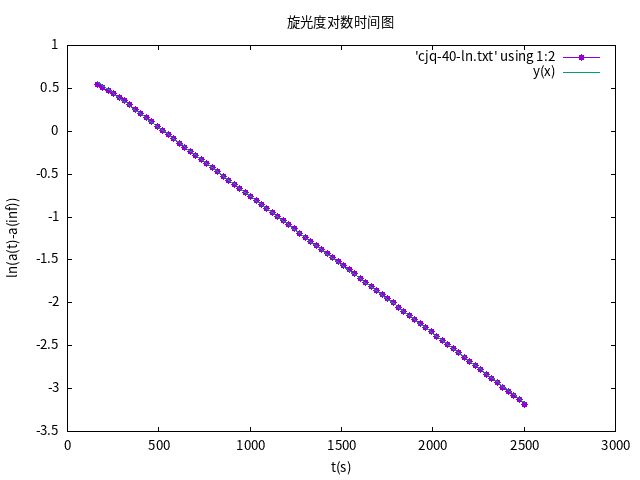
\includegraphics[width=.9\linewidth]{../data/cjq-40-ln.png}
\end{center}
拟合结果如下:
\begin{verbatim}
After 6 iterations the fit converged.
final sum of squares of residuals : 0.0059991
rel. change during last iteration : -9.33636e-08

degrees of freedom    (FIT_NDF)                        : 77
rms of residuals      (FIT_STDFIT) = sqrt(WSSR/ndf)    : 0.00882669
variance of residuals (reduced chisquare) = WSSR/ndf   : 7.79104e-05

Final set of parameters            Asymptotic Standard Error
=======================            ==========================
k               = -0.00160037      +/- 1.452e-06    (0.09071%)
b               = 0.844622         +/- 0.002174     (0.2574%)

correlation matrix of the fit parameters:
#                k      b      
k               1.000 
b              -0.890  1.000 

\end{verbatim}
拟合直线的斜率k为-0.001600(s\textsuperscript{-1}),所以
\[
t_{1/2}=\frac{\ln 2}{|k|}=\frac{\ln 2}{0.001600}=433.22(s)
\]
\end{enumerate}

\section{表观活化能的计算}
\label{sec:orga4a1a8c}
由公式
\[
\ln\frac{k_{1}}{k_{2}}=-\frac{E_{a}}{R}\cdot \left(\frac{1}{T_{2}}-\frac{1}{T_{1}}\right)
\]
得
\[
E_{a}=-\frac{R\ln \frac{k_{1}}{k_{2}}}{\frac{1}{T_{2}}-\frac{1}{T_{1}}}=-\frac{R\cdot \ln\frac{0.001600}{0.000830}}{\frac{1}{273.15+40}-\frac{1}{273.15+35}}=105.312(kJ\cdot mol^{-1})
\]
\section{小组数据整合}
\label{sec:org3d0171c}
\begin{center}
\begin{tabular}{lrrrrrr}
组别 & T(\textsuperscript{o}C) & 蔗糖(10g/L) & HCl(mol/L) & k(s\textsuperscript{-1}) & \(\qt\) (s) & \(E_{a}\) (kJ/mol)\\
\hline
1(向思佳) & 30 & 5 & 2 & 0.000381 & 1812.0 & 97.214\\
2(向思佳) & 40 & 5 & 2 & 0.001304 & 468.0 & 97.214\\
3(艾姆拉) & 30 & 10 & 4 & 0.001730 & 400.8 & 85.399\\
4(艾姆拉) & 35 & 10 & 4 & 0.002998 & 231.0 & 85.399\\
5(刘煜超) & 30 & 5 & 4 & 0.001350 & 513.4 & 110.970\\
6(刘煜超) & 35 & 5 & 4 & 0.002760 & 291.7 & 110.970\\
7(周靖辰) & 30 & 10 & 2 & 0.001172 & 1362.6 & 129.500\\
8(周靖辰) & 35 & 10 & 2 & 0.000509 & 591.5 & 129.500\\
9(曹嘉祺) & 35 & 5 & 2 & 0.000830 & 834.0 & 105.312\\
10(曹嘉祺) & 40 & 5 & 2 & 0.001600 & 433.2 & 105.312\\
\end{tabular}
\end{center}
\[
\overline{E_{a}}=105.679kJ\cdot mol^{-1}
\]
\end{document}
